\section{Reflexion}

\subsection{Reflexionsgesetz}

\begin{minipage}[c]{0.42\columnwidth}
    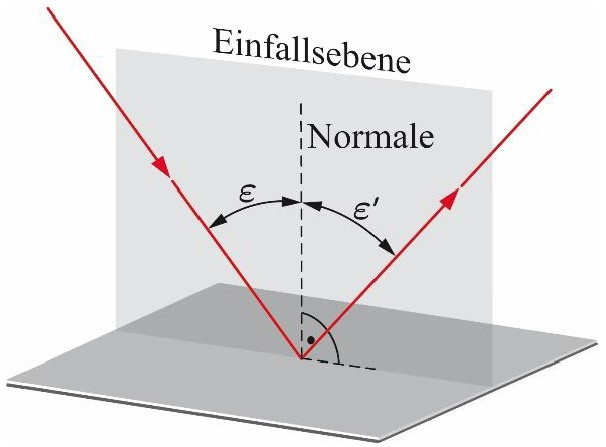
\includegraphics[width=\columnwidth]{images/reflexionsgesetz.jpg}
\end{minipage}
\hfill
\begin{minipage}[c]{0.48\columnwidth}
    \begin{center}
        Einfallswinkel = Ausfallswinkel 
    \end{center}
    $$ \boxed{ \varepsilon = \varepsilon' } $$
\end{minipage}


\subsubsection{Grenzflächen von Reflexionen}

\begin{minipage}{0.4\columnwidth}
    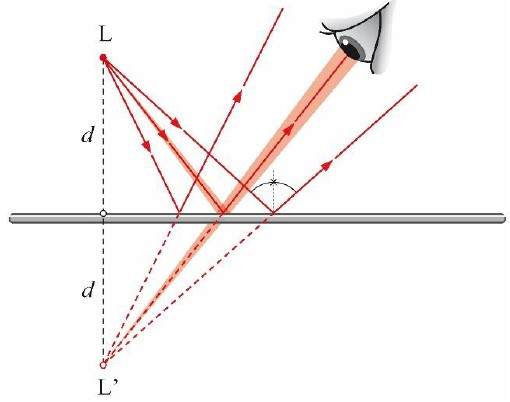
\includegraphics[width=\columnwidth]{images/reflexion.jpg}
\end{minipage}
\hfill
\begin{minipage}{0.58\columnwidth}
    \begin{tabularx}{\columnwidth}{l X}
    $L$ & reelles Bild \\
        & Bild, welches auf Schirm abgebildet werden kann \\
        & \\
    $L'$& virtuelles Bild (Spiegelbild von $L$)\\
        & Bild, welches nicht auf Schirm abgebildet werden kann 
    \end{tabularx}
\end{minipage}

\begin{description}
    \item[Glatter Spiegel:] direkte Reflexion (siehe Bild oben)
    \item[Rauer Spiegel:] diffuse Refelxion
\end{description}



\subsection{Reflexionen -- Spezialfälle}

\begin{tabularx}{\columnwidth}{l X}
    Brennpunkt $F$  & Brennpunkt (Fokus) ist der Punkt, in dem parallel zur optischen Achse auf einen Spiegel oder eine Linse einfallende Stahlen sich schneiden    \\
                    &                                                                                                                                               \\
    Brennweite $f$  & Abstand des Brennpunktes von der Linse bzw. dem Spiegel
\end{tabularx}


\subsubsection{Parabolspiegel}

Parallel einfallende Strahlen werden in einem Punkt fokussiert.

\medskip

\begin{minipage}[c]{0.8\columnwidth}
    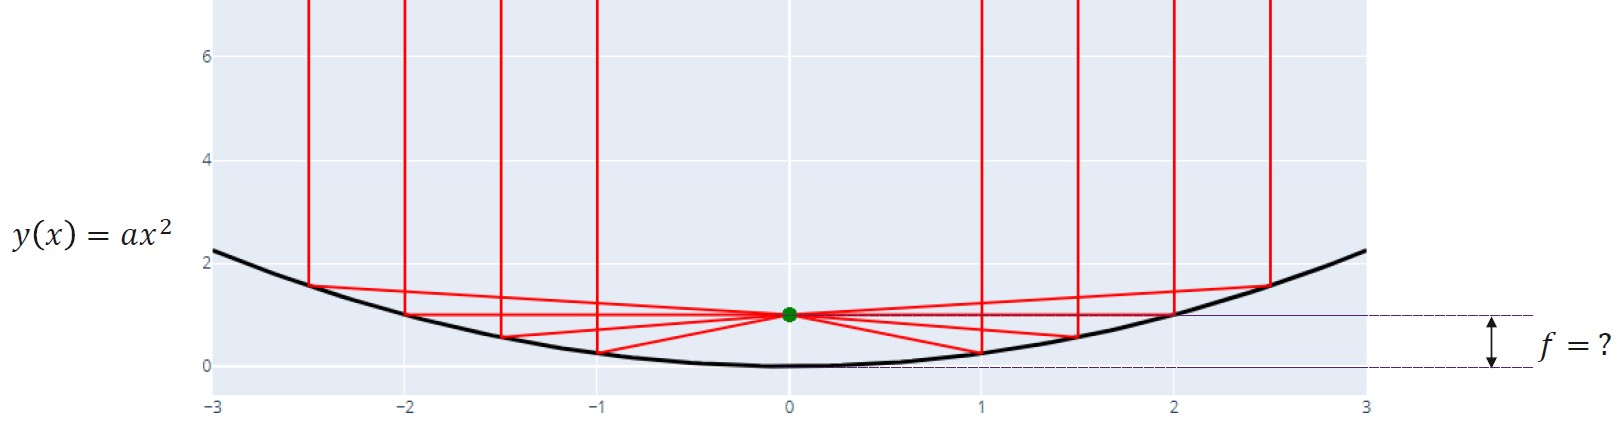
\includegraphics[width=\columnwidth]{images/parabolspiegel.jpg}
\end{minipage}
\hfill
\begin{minipage}[c]{0.18\columnwidth}
    $$ \boxed{ y(x) = a \, x^2 }$$ 
    $$ \boxed{ f = \frac{1}{4 \, a} } $$ 
\end{minipage}


\subsubsection{Elliptischer Spiegel}

Konzentration von Energie in einem nicht zugänglichen Punkt 

\begin{minipage}[t]{0.48\columnwidth}
    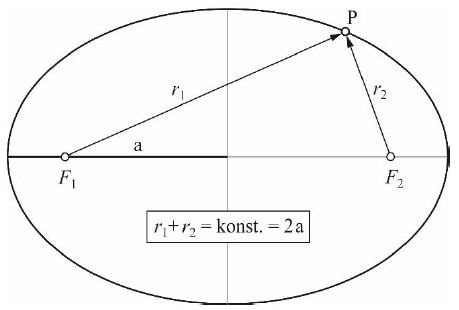
\includegraphics[width=\columnwidth, align=t]{images/elliptischer_spiegel.jpg}
\end{minipage}
\hfill
\begin{minipage}[t]{0.48\columnwidth}
    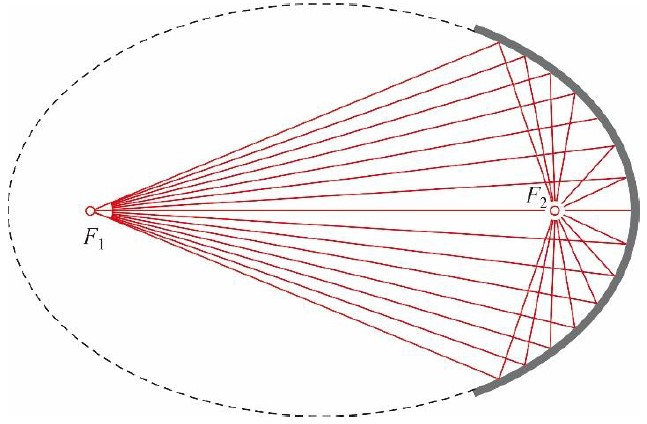
\includegraphics[width=\columnwidth, align=t]{images/elliptischer_spiegel_2.jpg} 
\end{minipage}

$$ \boxed{ y(x) = \frac{x^2}{a^2} + \frac{y^2}{b^2} } $$


\subsubsection{Hyperbolischer Spiegel}

Objekt in Spiegel versetzen 

\begin{minipage}{0.4\columnwidth}
    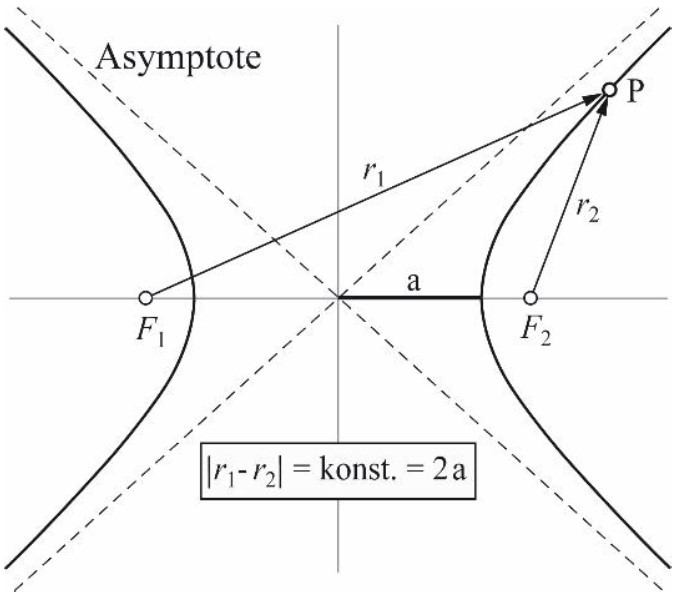
\includegraphics[width=\columnwidth]{images/hyperbolischer_spiegel.jpg} 
\end{minipage}
\hfill
\begin{minipage}{0.48\columnwidth}
    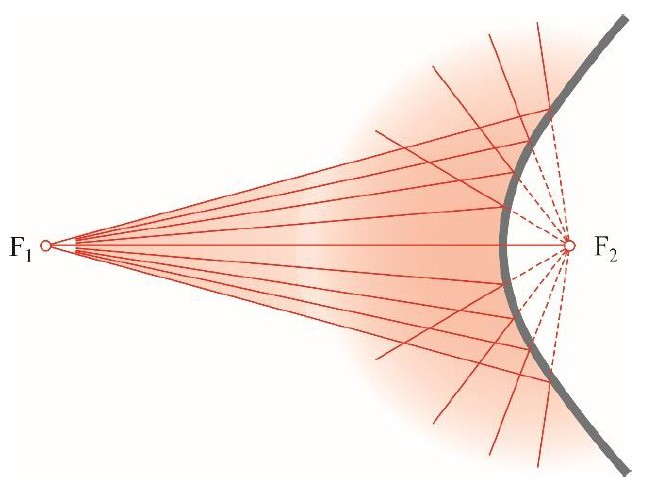
\includegraphics[width=\columnwidth]{images/hyperbolischer_spiegel_2.jpg} 
\end{minipage}

$$ \boxed{ \frac{x^2}{a^2} - \frac{y^2}{b^2} = 1} $$


\subsubsection{Sphärische Spiegel}

Parallel einfallende Stahlen werden nicht mehr in einem Punkt fokussiert (Katakaustik) 

\smallskip

Da die achsnahen Strahlen nach der Reflexion annähernd durch einen Punkt gehen, wird dieser Punkt wieder Brennpunkt $F$ genannt.

\begin{center}
    \begin{minipage}{0.4\columnwidth}
        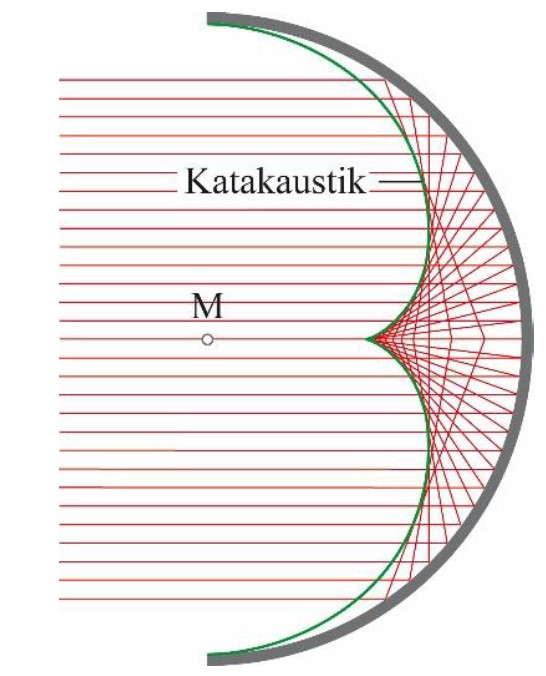
\includegraphics[height=3.5cm]{images/sphaerischer_spiegel_2.jpg}
    \end{minipage}
    \begin{minipage}{0.45\columnwidth}
        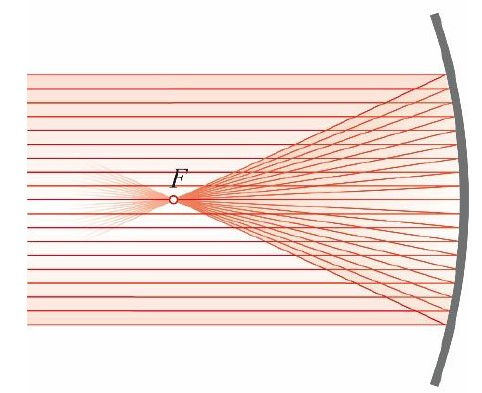
\includegraphics[height=3.5cm]{images/sphaerischer_spiegel.jpg}
    \end{minipage}
\end{center}

\vspace{-0.3cm}

\begin{minipage}[c]{0.2\columnwidth}
    $$ \boxed{ f = \frac{r}{2} } $$
    \smallskip
\end{minipage}
\hfill
\begin{minipage}[c]{0.76\columnwidth}
    \begin{tabular}{clc}
        $f$ & Brennweite                    & $[f] = \meter$    \\
        $r$ & Krümmungsradius des Spiegels  & $[r] = \meter$    \\
    \end{tabular}
\end{minipage}

\vspace{-0.3cm}

